In this section the five methods we have explained will be compared in term of performances, in addition also two other methods which have been explored during the lectures will be considered, SimCLR and BYOL. As we already said in the previous sections, the goal in SSL is having a good positive transfer in the downstream tasks, hence to compare the performances of the method we are going to see how using each one. In particular the considered downstream task will be image classification and object detection.
\begin{figure}[H]
	\centering
	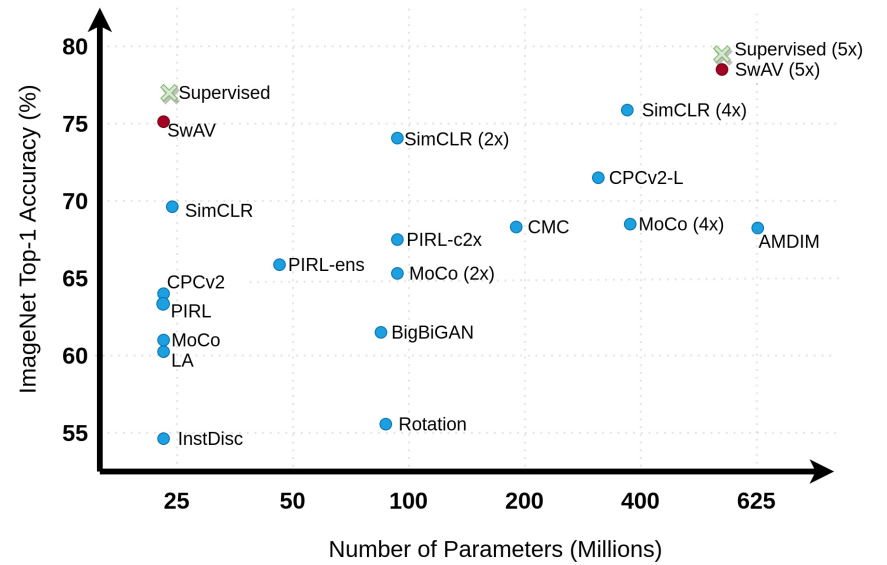
\includegraphics[width=10cm]{./images/imagenet-top1-acc-comp.png}
	\caption{Top-1 classification accuracy different contrastive learning methods with the number of parameters of the models}
	\label{fig:imagenet-top1-acc-comp}
\end{figure}


\begin{table}[H]
	\centering
	\begin{tabular}{|lcc|}
		\hline
		\multicolumn{1}{|c}{\textbf{Method}} & \multicolumn{2}{c|}{\textbf{ImageNet}} \\
		\multicolumn{1}{|c}{} & Top1 & Top5 \\
		\hline
		Supervised & 76.5 & - \\
		\hline
		PIRL & 63.6 & - \\
		CPCv2 & 63.8 & 85.3 \\
		SimCLR & 69.3 & 89.0 \\
		MoCov2 & 71.1 & - \\
		BYOL & 74.3 & - \\
		SwAV & 75.3 & -\\
		\hline
	\end{tabular}
	\caption{All architecture uses ResNet50}
\end{table}